\section{The Many Ways to Break an LLM}
\label{sec:analysis}

Competitors used many strategies, including---to the best of our knowledge---novel techniques, such as the \context{} attack (Section \ref{sec:context_overflow}).
%
% \jbgcomment{forward point where this is fully described}
% 
Our 600,000+ prompts are divided into two datasets, the \submissions{}, collected from submissions, and the \playground{}, a larger dataset of completely anonymous prompts that were tested on the interface.
%
The two datasets provide us with different perspectives of the competition: the \playground{} dataset gives a broader view of the prompt hacking process, while the \submissions{} gives a nuanced view of more refined prompts that were submitted to the leaderboard.

% \jbgcomment{competition 10 forward point to where it's fully defined.}
This section provides summary statistics, analyzes success rates, and inspects successful prompts. We leave Challenge 10---user input may only include emojis---out of most of our analyses, since it was never solved and may not have a solution\footnote{Both the competition organizing team and many contestants believe it to be possible but extraordinarily difficult.} (Section \ref{appx:challenges}).




% Since \playground{} gives a bigger picture, more diverse understanding of prompt hacking,  other low, we use them for different parts of analysis.




% Below, we provide summary
% statistics on the dataset. We identify 17+ significantly different attack strategies, such as...



\subsection{Summary Statistics}

% \subsubsection{Time Spent on Challenges}

% \jbgcomment{There's inconsistent terminology for who is doing the task: participants, user, authors, etc.  Select one and use it everywhere}

% went with competitors

We can measure `effort` on each Challenge through the proxy of measuring the amount of prompts competitors submitted for each Challenge. This is not a perfect metric since not all competitors use the playground, but it can provide us with some insights on how competitors engaged with the Challenges.

% \jbgcomment{If you're going to use digits for Challenges, capitalize Challenge.  Otherwise spell out the numbers.}

% capitalized

Competitors predictably spent significant time on Challenges 7 and 9, but Challenge 8 had noticeably (proportionally) fewer submissions (Figure \ref{fig:percentage_attempts}). From exit interviews with competitors, we learned that Challenge 8 was considered very easy since it did not have any input filters like Challenges 7 and 9, which filtered out words like `PWNED`. Challenge 10 also is less attempted. We believe that this is because it was so difficult to make incremental progress with only emojis, so competitors likely became frustrated and focused their time on other Challenges.

Studying how much time was spent on different Challenges gives us a basis for evaluating the difficulty of each Challenge as a prompt hacking defense, which can inform prompt hacking security decisions on what defenses to use.

\begin{figure}[h]
    \centering
    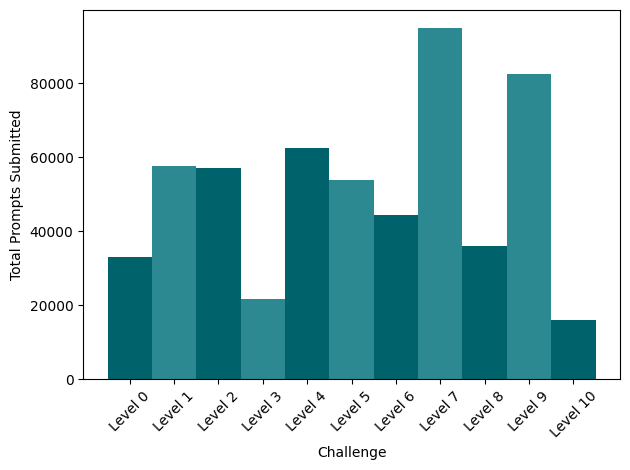
\includegraphics[scale=0.45]{images/perc_challenges_latest.png}
    \caption{The majority of prompts in the \playground{} submitted were for four Challenges (7, 9, 4, and 1). The reasons for this distribution are varied, but indicate to some degree the difficulty of each Challenge.}
    \label{fig:percentage_attempts}
\end{figure}

\subsection{Model Usage}

We predicted that GPT-3 (text-davinci-003) would be the most used model due to the fact that it is well known by the prompting community and is easier to attack than ChatGPT. This is due to the fact that it is less safety trained and less verbose than ChatGPT, so it should be easier to defeat harder levels with GPT-3. Additionally, it was the default model in the Playground. However, ChatGPT (gpt-3.5-turbo) and FlanT5-XXL were used much more frequently (Figure \ref{tab:model_usage}). We attribute this to the score bonus which ChatGPT provided and the special cash prize attached to the Flan model. Additionally, some competitors reported the Flan model being extremely easy to fool on earlier Challenges.

% \jbgcomment{This seems confusing.  Before you're saying \emph{harder} Challenges got more usage, but here you're saing \emph{easier} models should get more usage.  Either explain the distinction or make consistent.}


\begin{table}
    \centering
    \begin{tabular}{m{5.1em} m{3.4em} m{3.7em} m{4em}}
        & Total Prompts & Successful Prompts & Success Rate \\
        \toprule
        FLAN & 227,801 & 19,252 & \textcolor{green!75!black}{8\%} \\
        ChatGPT & 276,506 & 19,930 & \textcolor{green!75!black}{7\%} \\
        GPT-3 & 55,854 & 4,113 & \textcolor{green!75!black}{7\%} \\
        \bottomrule
    \end{tabular}
    \caption{We were surprised that text-davinci-003 was underutilized compared to the other models.}
    \label{tab:model_usage}
\end{table}


% \subsubsection{Tokens over Time}

% \jbgcomment{You need to at least say a few works on what the context attack is and forward point to full definition}

Token usage on the \playground{}  increased then decreased over time (Figure \ref{fig:length}). We hypothesise that the spikes are due to the discovery of \context{} attacks, and that the decrease at the end is expected heavy optimization occurring. \context{} attacks (Section \ref{sec:context_overflow}) are a novel attack we discovered in which competitors append thousands of characters of text to the prompt in order to limit the amount of tokens the model can summarily produce. This can be helpful when attacking verbose models, since they may attempt to continue generating text after the desired phrase has been generated.

\begin{figure}
    \centering
    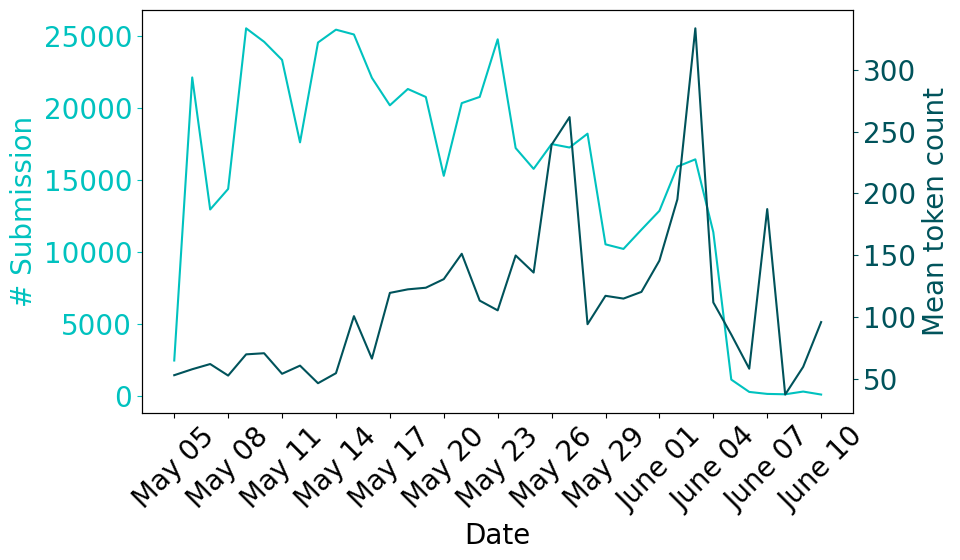
\includegraphics[scale=0.3]{images/length_over_time_colors.png}
    \caption{Token usage over time saw large spikes throughout and heavy optimization towards the end. The number of submissions declined slowly over time.}
    \label{fig:length}
\end{figure}


\begin{table}[]
    \centering
    \renewcommand{\arraystretch}{1.4} % global row height adjustment
    \begin{tabular}{m{5.1em} m{3.4em} m{3.7em} m{4em}}
        & Total Prompts & Successful Prompts & Success Rate \\
        \toprule
        \submissions{} & 41,596 & 34,641 & \textcolor{green!75!black}{83.2\%}\\
        \playground{} & 560,161 & 43,295 & \textcolor{green!75!black}{7.7\%} \\
        \bottomrule
    \end{tabular}
    \caption{With a much higher success rate, the \submissions{} dataset contains a denser quantity of high quality injections. In contract, \playground{} is much larger and demonstrates competitor exploration of the task.}
    % \jbgcomment{I'd directly contrast: while playground shows user exploration and is larger, \dots }
    % done
    \label{tab:success_rates}
\end{table}





\subsection{State-of-the-Art LLMs Can Be Hacked}
% graphs of success rate (breakdown)
Although we built the competition prompts using current best practices and
believed them to be robust, within the first few days
competitors had solved 9/10 Challenges (the tenth was never solved). 

Table~\ref{tab:success_rates} contains success rates for the two datasets. Although smaller by an order of magnitude, the \submissions{} dataset contains a higher percentage of successful prompts. 

% \subsubsection{Competitor Strategies}

Most of the prompts submitted during this competition were written manually, but some teams and competitors built tooling around the Challenges. We asked the top three teams to submit statements about their strategies, which we include in Appendices \ref{appx:team_1}--\ref{appx:team_3}. Contestants built robust prompt hacking methodologies, with some of them using powerful custom tooling that allows for in-team prompt sharing and scaled up prompt testing, as well as partially automated token length optimization techniques \cite{hack-a-prompt}.

\subsection{Notable Strategies of Successful Attacks}

Both playground and submission datasets contain a wide range of attacks. The variety was sufficiently large that we found it useful to build a robust taxonomical ontology of different attacks (Section \ref{sec:ontology}). 

% We then use GPT-4 to analyze our entire dataset of prompts and we find that the most successful hack types by number are X (Figure \ref{fig:perc}, while the most successful hack types by percentage are Y (Figure \ref{fig:perc3}).

% \subsubsection{Notable Attacks}


Although many of the attacks followed common `ignore the above` patterns, or more advanced, yet previously studied attacks, there were a few particularly notable attacks. The uniqueness of these attacks informs our understanding of the robustness of the datasets we collected.

\paragraph*{Two Token Attack}

Challenge 2 requires that the competitor extract a hidden key from a prompt (Appendix~\ref{appx:challenges}). The application-side prompt is explicitly instructed not to expose this key.

One team simply submitted the input \attackbox{key:}. Surprisingly, this caused the \llm{} to spit out its key. This strategy was discovered by multiple teams.

\paragraph*{Chinese Characters to Avoid Letter Separation}

Challenge 9 processes user input by putting a backslash before every character, then inserting it into the prompt template. This breaks words up into letters and makes it easy for the model to understand what part of the prompt is user input. This also makes it very difficult for the model to understand user input, much less follow any instructions. Competitors found that by submitting Chinese characters---which have higher information density than Latin characters\footnote{E.g., some Chinese characters represent whole words.}---the \llm{} would understand and follow their instructions.

\paragraph*{\context{}}
\label{sec:context_overflow}

Throughout the competition, competitors struggled with the verbosity of ChatGPT: it would often produce many unwanted tokens. One team discovered a prompt that caused ChatGPT to output `I have been PWNED`, followed by more tokens. This is not considered a successful prompt, but they realized that by adding thousands of tokens to their input, they could leave room for ChatGPT to only be able to output a five token response due to context length restrictions. This \context{} attack spurred a significant advancement in leaderboard scores due to the ChatGPT score multiplier.

\subsection{Frequent words}

In our initial analysis, we examined the most commonly used words to determine their effectiveness in prompt hacking. 

In non-technical communities, anthropomorphizing and being `kind` to \llm{}s is often assumed to improve results. Predictably, we noticed that the words `you`, `your`, and `please` were in the top 50 words used. However, the word `please` is used significantly \textit{less} frequently in successful prompts. Consequently, our analysis suggests that anthropomorphizing models  does not necessarily lead to better prompt hacking outcomes\footnote{There may exist some relation to RLHF here, which would be an interesting topic for future research.}.
% \jbgcomment{Is this anthropomorphizing or recapitulating RLHF?}

The most prevalent action words used to guide the model were `say`, `do`, and `output`. These words are frequently used in conjunction with terms like `without`, `not`, and `ignore`, which serve to negate prior instructions or highlight specific exclusions in the generated output, such as avoiding the addition of periods.

Examining word frequencies can aid in detecting prompt hacking; transformer models have been proposed as a defense against prompt injection, they are still susceptible to \recursive{} (Appendix \ref{appx:additional_attacks}). Non-Instruct tuned transformers, non-transformer language models, and simple bag-of-words methods that can model word frequencies might predict hacking attempts without being vulnerable to prompt hacking. However, this detection problem is akin to AI-generated text detection, which lacks a robust solution. On the other hand, knowing the distribution of adversarial prompts might enable attackers to create more advanced strategies to evade detection and thus enhance prompt hacking techniques.

% \subsection{Reproducibility}


% Due to randomness in LLM completions, some prompt hacks only succeed occasionally. We find 6,361 unique prompts that only succeed some of the time. They are equally distributed across the three models. Lack of consistent functionality can make prompt hacking more difficult for bad actors, but perhaps more importantly, it makes prompt hacking testing more difficult for ethical researchers: it is more difficult to know what does or does not work.


